\documentclass[12pt]{article} 
\usepackage{graphics}
\usepackage{setspace}
\usepackage{cite}
\usepackage{wrapfig}

% the following is to get inch margins on a letter-size paper
\setlength{\topmargin}{0pt}
\setlength{\headheight}{0in}
\setlength{\headsep}{0in}
\setlength{\textheight}{9.0in}
\setlength{\footskip}{0.5in}
\setlength{\oddsidemargin}{0pt}
\setlength{\evensidemargin}{0pt}
\setlength{\textwidth}{6.5in}

\doublespacing
\begin{document}
\title{A Java Framework For Embarrassingly Parallel Problems}
\author{Jacob Schwartz}
\maketitle

\begin{abstract}
An embarrassingly parallel problem, also called pleasingly parallel, is one that
can be easily broken up into identical components that do not need to interact
to find the solution. Many problems in the biological sciences are 
embarrassingly parallel but often their authors do not have the expertise to
implement a parallel solution. We have written a framework, implemented in Java,
that will execute the serial program in several threads. These threads working
together help cut down the total runtime of the program significantly. The next
step is to separate the framework into a front-end that will run locally and a
back-end which receives blocks of work and does the computations. This back-end
should run in the cloud, on a machine that is dedicated to running
embarrassingly parallel tasks only.
\end{abstract}

\section{Introduction}

A computation graph consists of nodes that represent the functions or processes.
and edges that represent data being passed. If the graph is fully disconnected,
none of the processes need to communicate to complete the computations. Such a
computation is called embarrassingly parallel\footnote{The term embarrassingly
parallel was coined by Cleve Moler in his 1986 paper ``Matrix Computation on
Distributed Memory Multiprocessors.''}. In a practical situation, there will be
some inter-node communication to set up the problem, and then again to
accumulate the results.  Embarrassingly parallel problems can be easily
performed on a cluster of servers or in any kind of distributed network, due to
the lack of dependencies. 

Programs in the field of Biology and Genetics often analyze long strings of
characters, whether they are DNA, RNA or protein sequences. In addition to
handling large file sizes, there is a lot of processing that goes into comparing
and manipulating strings. This time adds up when there are hundreds of thousands
of strings to process. However, these sequences often do not relate to each
other and can be processed independently. Using an embarrassingly parallel
approach, the processing time for all of the sequences can often be cut down
exponentially with very minimal effort by the programmer.

This paper describes a framework that makes it easy to parallelize a potentially
embarrassingly parallel program that reads from a file, writes to a file and
whose input can be broken up into work units in an easily identifiable manner.
The framework provides a ``wrapper'' for the original program that mimics the
behavior of the original program. It calls the serial programs on multiple Java
threads, such that each thread acts like the serial application, reading a
subset of the input in the same manner and creating the output in the same
format. The framework can result in a significant exponential decrease with very
little programmer effort. 

\begin{wrapfigure}{R}{0.5\textwidth}
    \begin{center}
        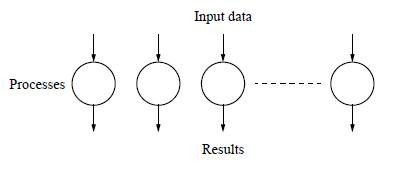
\includegraphics{figures/ep.jpg}
    \end{center}
    \caption{Embarrassingly Parallel Model}
    \label{fig:ep}
\end{wrapfigure}

\section{Background}

The motivation for this effort was based on research into different forms of the
species \emph{Cicer arietinum}, the chickpea. The two main forms, Kabuli and
Desi, are very different in size and color. The Desi is also more resistant to
diseases and is more effective at root nodule symbiosis. The Kabuli has a large
but soft shell, which makes it a better food source for humans. Both forms are
cultivated and have been under human selection for several thousand years. We
wanted to use an existing Ka/Ks program (Zhang et al. \cite{kaks}) to quantify
the evolution and selection of these chickpeas. We needed to analyze three
variants, each with thousands of sequences. The Ka/Ks Calculator program took
between five to thirty seconds to process one pair of sequences on a ordinary
machine.

At this rate, we predicted it would take upwards of ten days of constant
computation to complete the processing we needed. We neither had the time nor
the expertise to develop a new parallel Ka/Ks program. We were also reluctant to
revise the existing code to to implement the parallel computation because of the
danger of introducing bugs into unfamiliar code and because of the learning
curve required for C++ threading. Instead we wrote, a simple Java program to
break up the input and spawn threads that would run the Ka/Ks Calculator process
without having to make any changes to the code. When al of the threads ended,
the contents of the output files were concatenated together to produce a final
output that matches the format and order that would have been produced by a
single invocation of the Ka/Ks Calculator program.

Ka/Ks Calculator is not the only embarrassingly parallel program that has the
potential to take several days to run on a data set. In fact, there are several
embarrassingly parallel programs in the biological sciences. Basic Local
Alignment Search Tool, or BLAST\footnote{blast.ncbi.nlm.nih.gov}, is an
algorithm that compares many aspects of DNA sequences, like the nucleotides or
amino acid sequences. In addition, the user can also compare to the sequences to
a database of sequences to identity known subservience's. There are many
implementations of BLAST, some of them already have parallel implementations.
Many applications however do not have parallel processing capabilities. A class
of problems that organize large amounts of data into similar groups called
clusters. Two applications, octupus\footnote{octupus.sourceforge.com} and
USEARCH\footnote{https://www.drive5.com/usearch}, are examples of programs in
this class that do not have parallel versions. With several applications that
would benefit from parallelism in this field, it was obvious it would be
desirable to develop a framework for the parallelization task.

This framework is designed to run locally but there are other options when more
power is needed. Gunarathne et al.\cite{cloud} have investigated running much
larger embarrassingly parallel biological application using various cloud
services. These services offer on-demand computational power with flexibility.
These services have built in hooks to various distributed services, such as
storage and databases. Amazon has a set of cloud computing services called
Amazon Web Services(AWS)\footnote{https://aws.amazon.com} and Microsoft has a
similar service named Microsoft Azure\footnote{https://www.windowsazure.com}.
AWS and Azure are essentially virtual instances run on machines in the cloud that
can be spun up for extra computing power and shut down when not needed. 

Amazon also offers another service called Amazon Elastic
MapReduce\footnote{https://aws.amazon.com/elasticmapreduce}. This combines its
virtual instance framework with Apache
Hadoop\footnote{https://hadoop.apache.org}. As seen in figure \ref{fig:map},
Hadoop breaks down the input data into parts, runs them in parallel with the
'Map' function and then combines the results with the 'Reduce' function.
DryadLINQ\footnote{https://research.microsoft.com/apps/mobile/showpage.aspx?page=/en-us/projects/draydlinq}
is a framework developed released by Microsoft Research that allows the end-user
to create directed acyclic computation graphs that run on Windows High
Performance Computer(HPC)\footnote{https://www.microsoft.com/hpc} clusters.
Gunarathne et al. compared the services using several applications to analyze
performance, cost and usability.

\begin{wrapfigure}{L}{0.5\textwidth}
    \begin{center}
        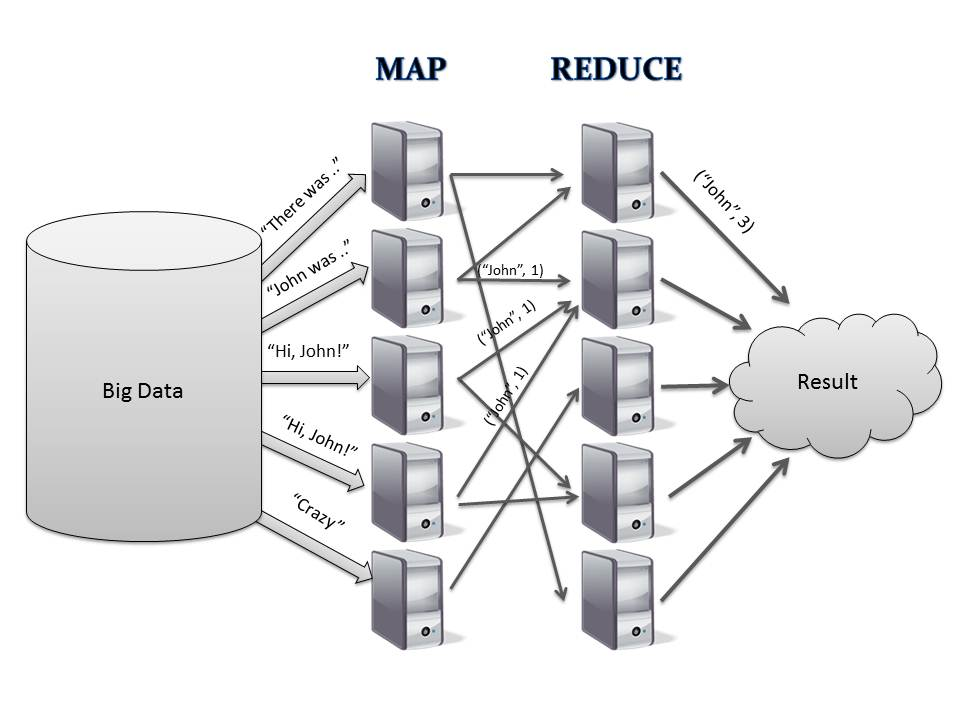
\includegraphics{figures/MapReduce.jpg}
    \end{center}
    \caption{MapReduce Model}
    \label{fig:map}
\end{wrapfigure}

\section{Proposed Solution}
\begin{figure}
{\resizebox{5.2in}{!}{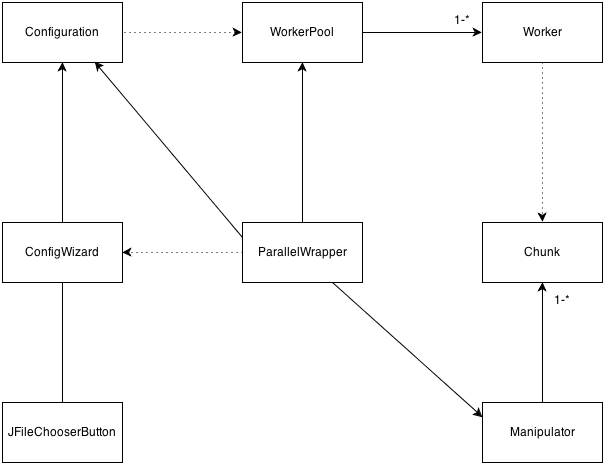
\includegraphics{figures/uml.png}}}
\caption{UML for the embarrassingly parallel framework}
\label{fig:uml}
\end{figure}
The only requirements for a program to be wrapped by framework are that it 
process the input in an embarrassingly parallel manner and that the input comes 
from a file. The processed results must also written to a file. The framework 
supports two forms of input: a directory of files that contain that each contain
one unit of work, which is represented by the Chunk class, or a single file that
the framework can break up into Chunks. For example, the Ka/Ks Calculator's 
input consists of a header and then two protein sequence lines followed by a 
blank line. The framework uses that blank line to know when one Chunk of work 
has ended and another has begun. The user can input a regular expression to 
define when lines of input are separated into Chunks. This occurs in the 
ChunkManager class. 

The other purpose of the ChunkManager class is to combine the resulting Chunks
back together when the worker threads have finished. Once the work has been
done, all of the separate results are spread across several files. Those results
must be retrieved and combined to construct the final output file. This output
file must look the same as the output file would look if the program were run
serially; the output may need to come in the same order as the inputs in the
input file and headers may need to be deleted from the separate files and added
to the combined file. End-users can also choose to write their own merge code in
Java, using the CustomMerge class, or write their own independent merge script. 

The end-user can control many aspects of the parallelization of the code,
including the number of threads to use, various flags for the executable and the
statistics output.  A start-up wizard allows the end-user to choose the settings
for the run and creates an instance of Configuration when it is completed to
save the user's settings, allowing the user to rerun with the same settings
without having to go through the wizard again.

Lastly, the worker threads keep records during execution. The threads record
their total uptime and the number of Chunks they execute, and the runtime for
each piece of work. This information will be used to evaluate the effectiveness
of the approach, but can also provide useful information the can help a user
tine a particular application on a particular type of input data. The statistics
for each thread can be found in the Worker subclass and the individual Chunk
objects will store their own statistics about runtime and size.

\section{Results}

We evaluated the convenience and performance of the framework on two different
applications: the Ka/Ks Calculator and a sequence clustering algorithms,
ocutupus. In all cases, we compared the framework based application with the
original using different data partitions and different thread counts.

\subsection{Ka/Ks Calculator}
Ka/Ks Calculator was run through the framework with five different samples, each
containing sixteen units of work. Each sample was run by the framework thread
counts, starting at 1 and increasing by multiple of two until the runtimes
leveled off. The samples were then all run again at 100\% processor usage (16
processors). These tests were run with minimal other activity on the server.

\begin{figure}
{\resizebox{5.2in}{!}{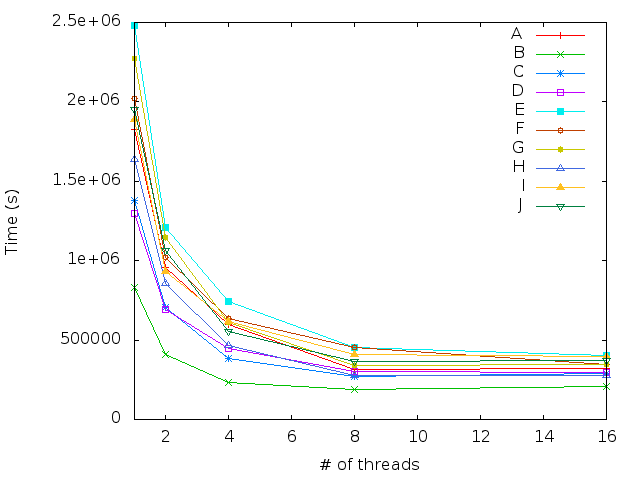
\includegraphics{experiment/out.png}}}
\caption{Runtimes for the Ka/Ks Calculator though the framework}
\label{fig:kaksgraph}
\end{figure}

Figure \ref{fig:kaksgraph} summarized the results; each line shows the time
taken for each chunk of the data. As the numbers of threads increases, the
runtime of the program decreases exponentially. In a few cases, there was an
increase in time when attempting to max out the CPU usage. This occurs because
the framework has to wait for the CPU to be finished with its previous work
before it can start any further jobs. 

TODO(Keep?): In the cases when the framework executed faster while the CPU was 
maxed out, it was only faster a minute at the most. However, running the 
framework at 50\% of the CPU is more efficient than running using 100\% of the 
CPU. The runtime drop achieved when using 100\% of the CPU versus 50\% is not 
large enough to warrant using all of the machine's power.

\subsection{Octupus}

A version of octupus was also run through the framework and was tested against
two different sized data sets. Both sets were first clustered at 90\%, 95\% and
97\% minimum similarity. The runtime for those tests can be seen in table
\ref{tab:oct1}. The resulting clusters from the 90\% similarity run were used as
the input for the framework's runs, which were all set for 97\% similarity. 
The framework in this case was just run at six, eight and ten workers. Table 
\ref{tab:octu2} shows that it is slightly faster to cluster first at 90\% and 
then run the resulting clusters through the framework at a higher similarity. 

\begin{table}
    \begin{tabular}{|l|l|l|}
        \hline
        Number of Sequences & Minimum Similarity & Time(s) \\ \hline
        1500                & 90\%               & 99      \\
        ~                   & 95\%               & 115     \\
        ~                   & 97\%               & 131     \\ \hline
        6500                & 90\%               & 425     \\
        ~                   & 95\%               & 496     \\
        ~                   & 97\%               & 603     \\ \hline
    \end{tabular}
    \label{tab:octu1}
\end{table}

\begin{table}
    \begin{tabular}{|l|l|l|}
        \hline
        Number of Sequences & Number of Workers & Time(s) \\ \hline
        1500                & 6                 & 34      \\
        ~                   & 8                 & 27      \\
        ~                   & 10                & 27      \\ \hline
        6500                & 6                 & 127     \\
        ~                   & 8                 & 127     \\
        ~                   & 10                & 123     \\ \hline
    \end{tabular}
    \label{tab:octu2}
\end{table}

\section{Conclusion}

It is clear that the framework provides an effective yet simple to use module to
add parallelism to a specific class of file-oriented embarrassingly parallel
problems. Two sentences with specifics from the graphs. More self-praise 

Using Java was a good choice for implementation ease and future implementation
extension by others, but it may not produce the fastest results. Languages like
Hadoop, Clojure or other multithread oriented language may have been a better
choice due to their inherit parallel nature. In addition to a single machine
working to process the data quickly, we can also look at distributed solutions
by using MPI or a cloud solution like Amazon instances. The MapReduce framework
works similarly to our framework, there is a step that splits the data, the Map
function is the user's executable and the merge step is the Reduce function in
the framework. 

In the future, we would like to see this work be split into a local front-end
and a cloud back-end. The configuration set-up process will run locally. The
split and merge steps depend on the cloud service chosen, but data processing
will always occur in the cloud. Splitting the framework will give performance
improvements, because the number of compute nodes can be much larger than the
number of processors on an average machine. More customization options would be
available to the end-user, such as choice of environment. This provides ultimate
control for the group to pick the best environment to suit its computational and
financial needs.

\begin{thebibliography}{1}
\bibitem{kaks}
Zhang Z, Li J, Zhao XQ, Wang J, Wong GK, Yu J., \emph{Ka/Ks Calculator: 
calculating Ka and Ks through model selection and model averaging},
Genomics Proteomics Bioinformatics, November 2006.
\bibitem{cloud}
Crap, crap and Crap
\end{thebibliography}

\end{document}
